\documentclass{article}
\usepackage[dvipdfm]{graphicx}
\usepackage[dvipdfm]{hyperref}


\title{SELinux Policy Editor Install Guide(for Ver 2.0))}
\begin{document}
\def\labelenumi{(\theenumi)}
\maketitle
\tableofcontents
\newpage

This document shows how to install SELinux Policy Editor.

\section{Install from RPMs}\label{sec:rpm}
Supported Platforms are Fedora Core5 and Cent OS 4.3(should work in Redhat
Enterprize Linux 4).\\

You can easily install from RPM
\begin{enumerate}
 \item Install required package\\
       You need checkpolicy package.
\begin{verbatim}
# yum install checkpolicy		
\end{verbatim}
And it is highly recommended to install audit package, and enable
       auditd.
\begin{verbatim}
#yum install audit
#chkconfig auditd on
#/etc/init.d/auditd start
\end{verbatim}


    \item Obtain files\\
Download seedit-converter-2.0.x.rpm and seedit-policy-2.0.x-(your
	  distro).rpm,seedit-gui-2.0.x.rpm, seedit-doc-2.0.x.rpm 
from below URL.
\begin{verbatim}
http://seedit.sourceforge.net/download.html
\end{verbatim}
If you use Fedora Core 5, download seedit-converter-2.0.x-FC5.rpm and
       seedit-policy-2.0.x-FC5.rpm.\\
If you do not have X Window System, you do not need seedit-gui package.

 \item Install rpms
Install rpm and restart by following commands.
\begin{verbatim}
$ su 
# rpm -ivh seedit-*.rpm
# reboot
\end{verbatim}
 \item Initialization\\ \label{item:init}
When system restarts, some relabeling process run. It takes some
	  minutes. When you log in, initialize policy and reboot again by following
	  command. 
\begin{verbatim}
# seedit-load
# reboot
\end{verbatim}
\item Notice about CentOS 4\\ 
If you are using CentOS4, there is a bug in SELinux's relabel command.
If you have installed strict policy, or have enabled RBAC before, 
you have to run following command.
\begin{verbatim}
# setfiles /etc/selinux/seedit/contexts/files/file_contexts  / -F -vv
# reboot
\end{verbatim}

 \item That's it!\\
You can make sure seedit is installed by following command.
\begin{verbatim}
# sestatus
SELinux status:                 enabled
Current mode:                   permissive
Mode from config file:          permissive
...
Policy from config file:        seedit
\end{verbatim}
Note that simplified policy is installed as {\it permissive} mode.
In {\it permissive} mode, SELinux is not protecting your system. It is
 only a test mode. To be a enforcing mode, see \ref{sec:mode}.\\
To make sure seedit is installed, go to section \ref{sec:makesure}.
\end{enumerate}

 \subsection{What's affected?}
 In this installation process ,
/etc/selinux/config is changed like below.
\begin{verbatim}
SELINUX=permissive	
SELINUXTYPE=seedit
\end{verbatim}
Our system does not interfere with other existing system components
except that.
\subsection{qUninstall}
If you want to uninstall. Do following.
\begin{verbatim}
# rpm -e seedit-policy seedit-converter	
# reboot
\end{verbatim}
You system will restart as SELinux targeted policy(Fedora Core5 default)
and permissive mode(SELinux is effectively disabled).



\section{Installing from source}
\begin{enumerate}
 \item Obtain files\\
Download seedit-converter-2.0.x.tgz and seedit-policy-2.0.x.tgz
From below URL.
\begin{verbatim}
http://sourceforge.net/project/showfiles.php?group_id=135756	
\end{verbatim}
 \item Build and install\\
\begin{verbatim}
# tar czvf seedit-*.tgz
# cd seedit-converter
# make install DISTRO=(FC5 or COS4)
# cd .. 
# cd seedit-policy
# make install DISTRO=(FC5 or COS4)
# cd seedit-gui
# make install
# touch /.autorelabel
# reboot
\end{verbatim}
Next is the same as \ref{sec:rpm} (\ref{item:init}).\\
 \item uninstall\\
You can go back to Fedora Core5 default by following.\\
Modify /etc/selinux/config like below.
\begin{verbatim}
SELINUXTYPE=seedit
-->
SELINUXTYPE=targeted
\end{verbatim}
And 
\begin{verbatim}
#touch /.autorelabel
#reboot	
\end{verbatim}
\end{enumerate}

\section{Make sure seedit is installed}\label{sec:makesure}

If you are using X Window System,  from  Gnome menu, 
. Choose Desktop $\rightarrow$ Manage $\rightarrow$ SELinux
Policy Editor.
You will see window like \ref{fig:controlpanel}
\begin{figure}
\caption{SELinux Policy Editor Control Panel}\label{fig:controlpanel}
\includegraphics*{images/controlpanel.png}
\end{figure}

Then  select {\it Status}, you will see \ref{fig:status-selinux}.
\begin{figure}
\caption{Status}\label{fig:status-selinux}
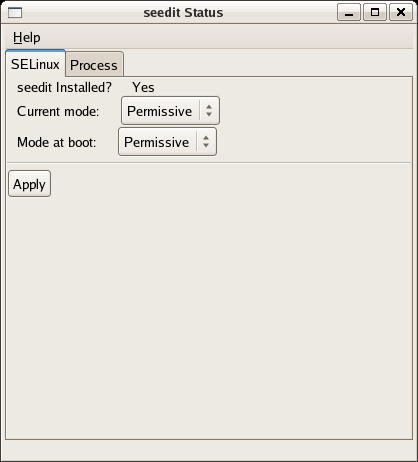
\includegraphics{images/status-selinux.png}
\end{figure}
If it shows {\it seedit installed: yes}, installation is success!.\\

From command line, if result of sestatus shows following, installation
is sucessful.
\begin{verbatim}
# sestatus
SELinux status:                 enabled
SELinuxfs mount:                /selinux
Current mode:                   permissive
Mode from config file:          permissive
...
Policy from config file:        seedit	
\end{verbatim}

Next,  see SELinux Policy Editor Administration Guide.

\end{document}